\chapter{Спукай балоните}

Целта на тази игра е за 30 секунди, играчът да спука максимално много балони. Играчът ще има катапулт, с помощта на който играчът ще пука балоните.

\begin{figure}[H]
  \centering
  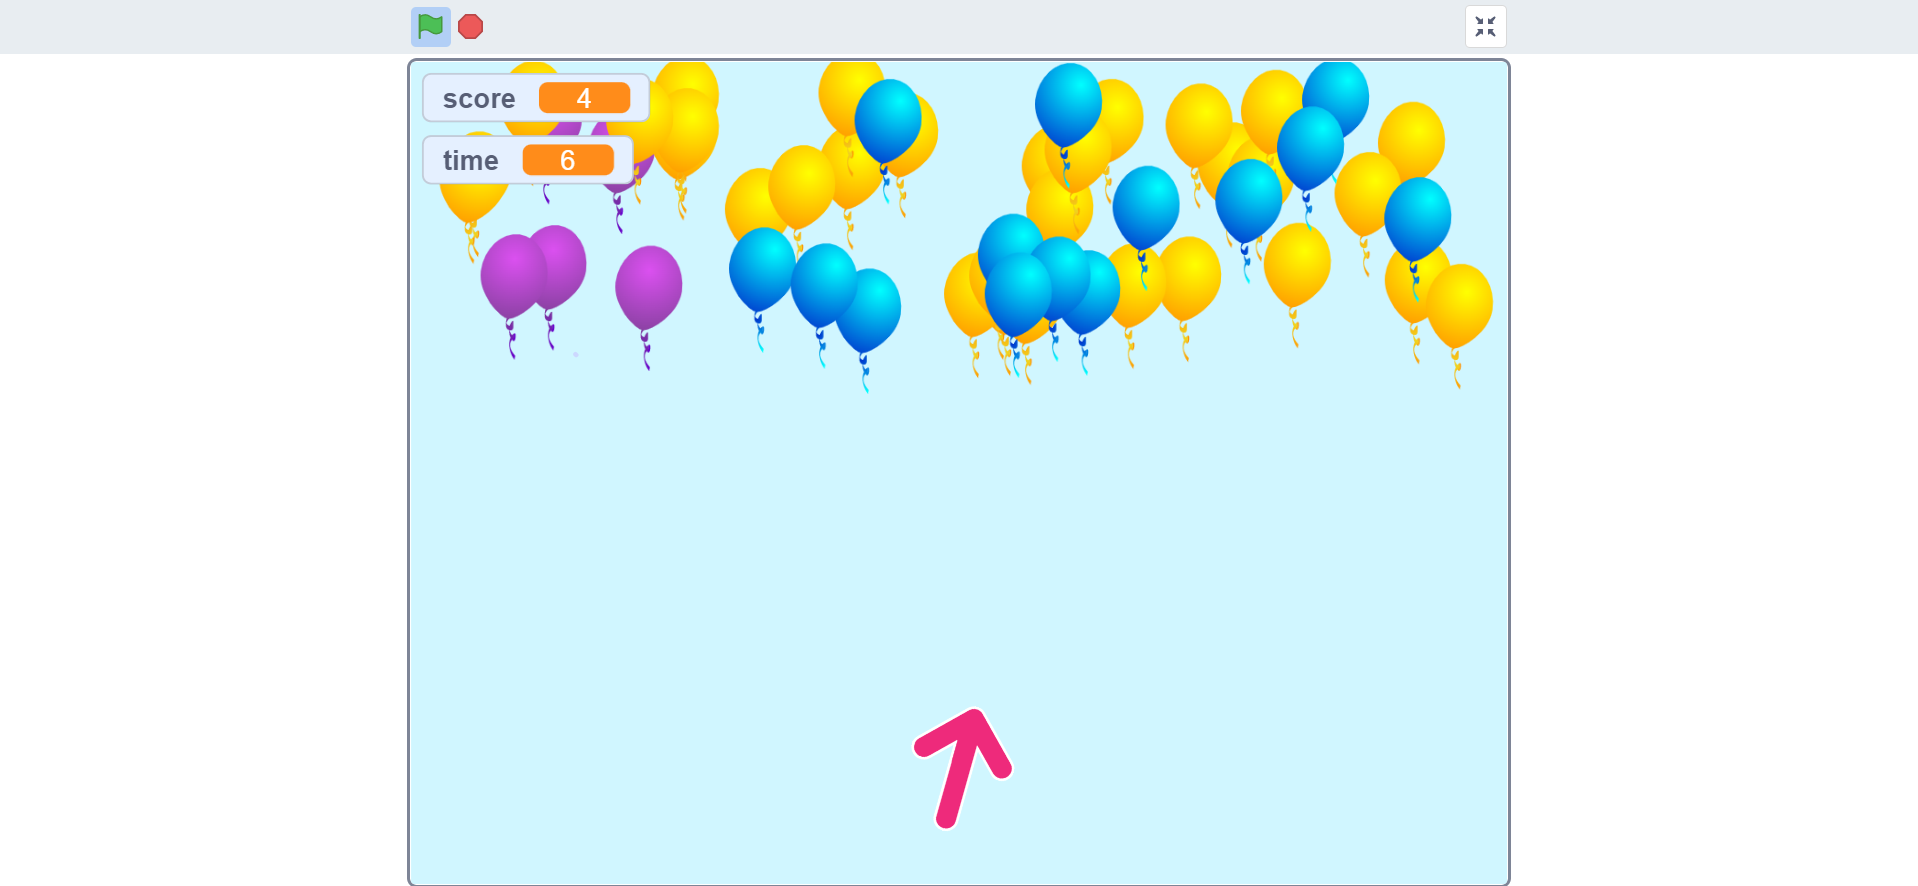
\includegraphics[width=1.0\linewidth,height=0.5\linewidth]{fig090001.png}
  \caption{Спукай балоните}
\label{fig090001}
\end{figure}

\section{Добавяне на фон и герои}
Първата стъпка от играта е да се изберат подходящ фон и герои. Необходимите герои в тази игра са стрелка, която ще представлява катапулта, балон и герой, който ще обяви резултатът, когато изтекат 30 секунди.

\begin{figure}[H]
  \centering
  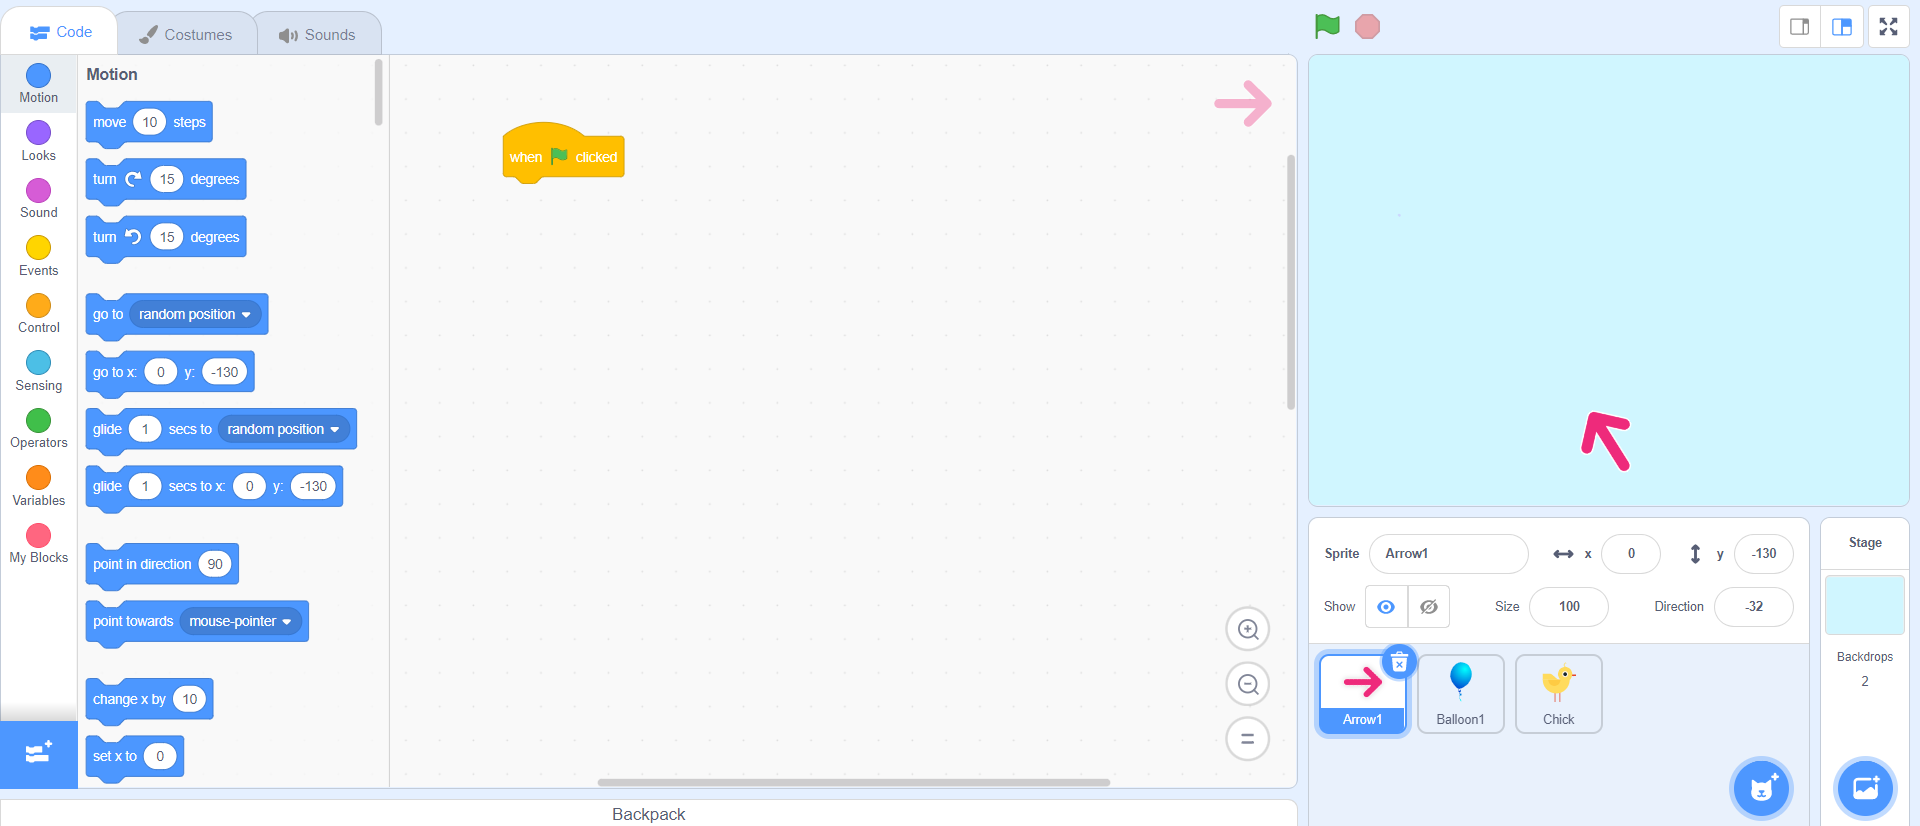
\includegraphics[width=1.0\linewidth,height=0.5\linewidth]{fig090002.png}
  \caption{Добавяне на фон и герои}
\label{fig090002}
\end{figure}

\section{Програмиране на катапулта}
В тази игра трябва да се дефинират две променливи - първата ще съхранява времето, а втората резултатът. В началото на играта първоначалната стойност на променливата време трябва да бъде 30, а стойността на променливата за резултатът трябва да бъде 0.

\begin{figure}[H]
  \centering
  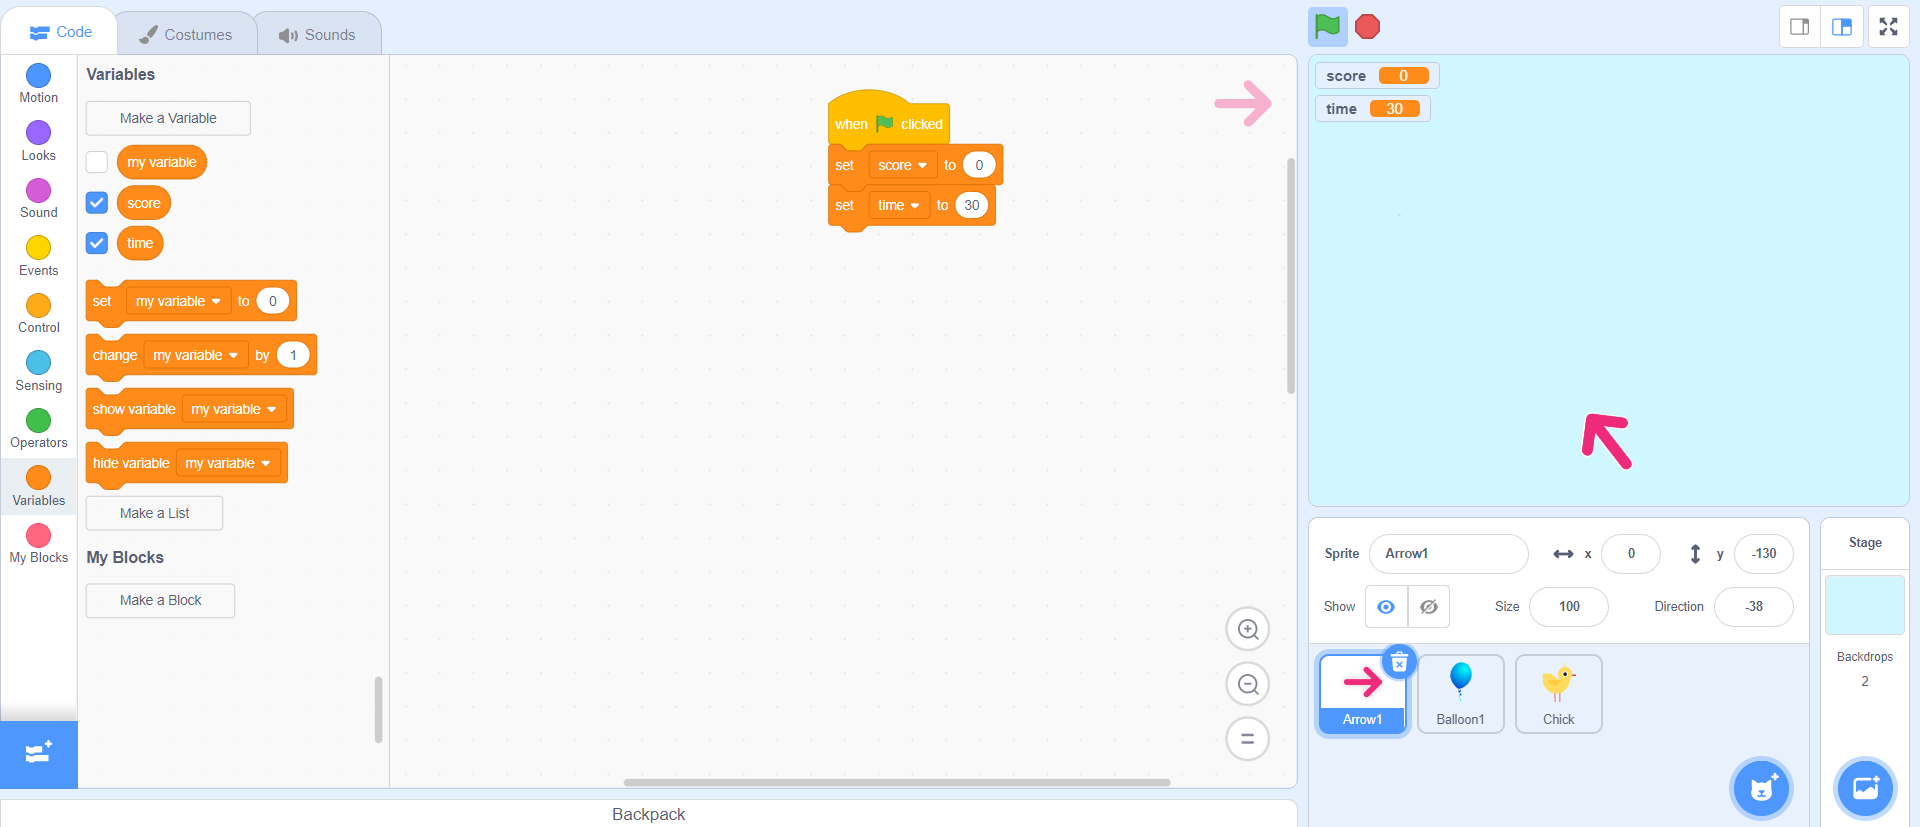
\includegraphics[width=1.0\linewidth,height=0.5\linewidth]{fig090003.png}
  \caption{Инициализиране на променливите}
\label{fig090003}
\end{figure}

Играта продължава докато променливата за време не стане равна на 0. Тя трябва да намалява стойността си през 1 секунда.

\begin{figure}[H]
  \centering
  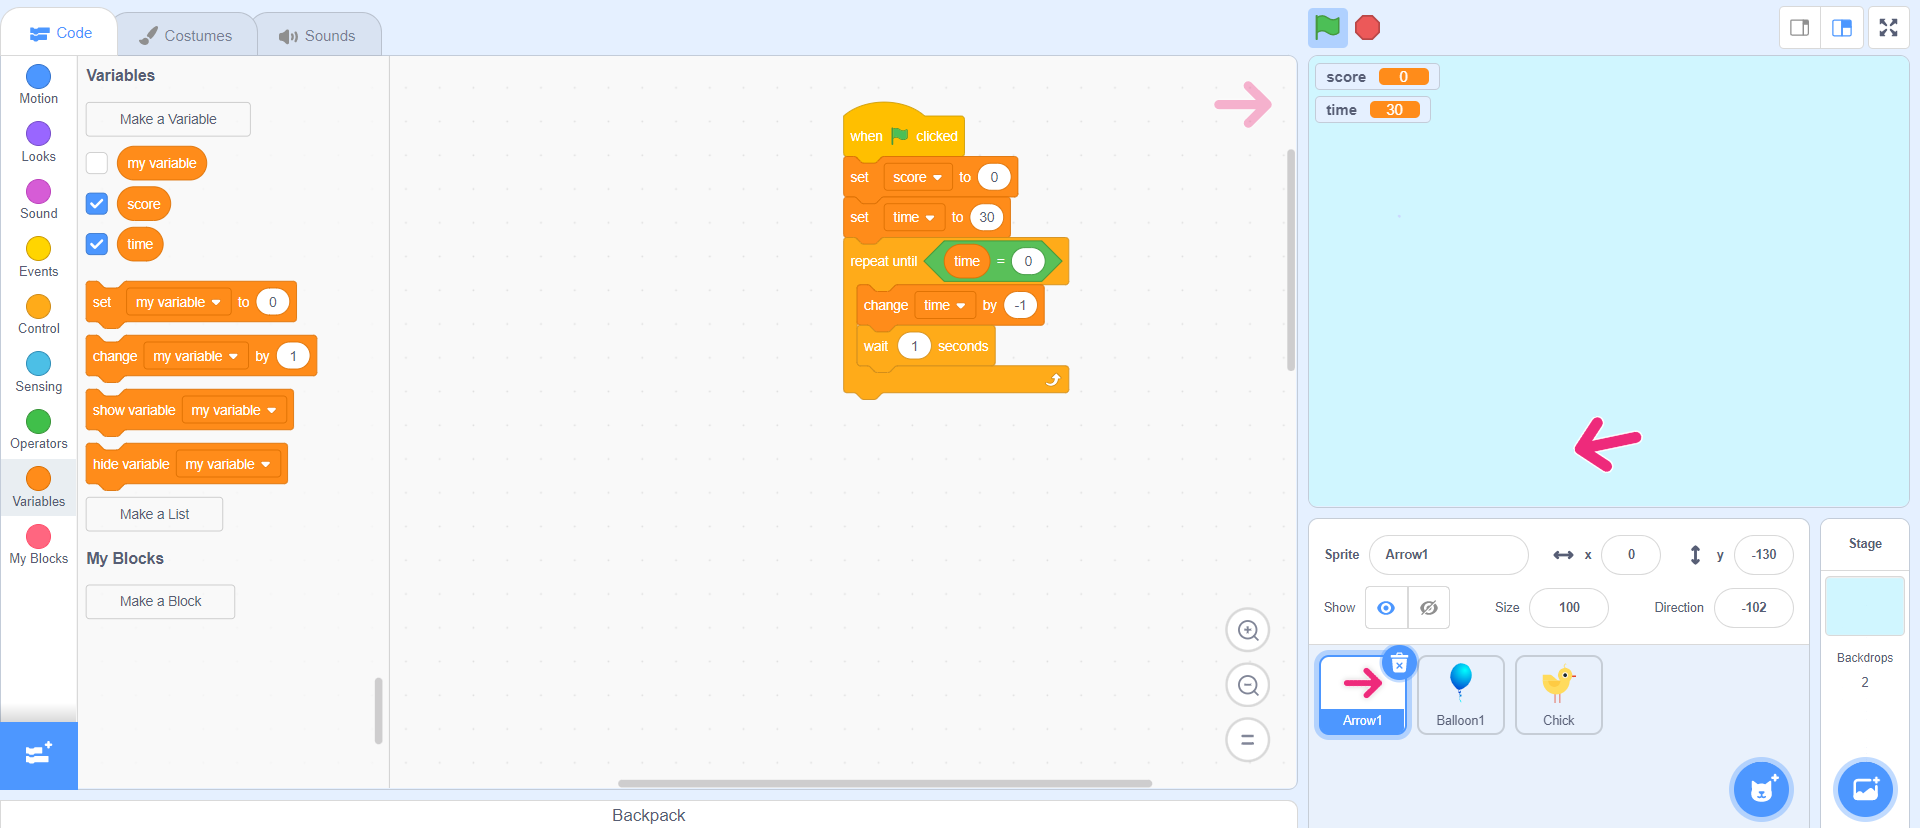
\includegraphics[width=1.0\linewidth,height=0.5\linewidth]{fig090004.png}
  \caption{Промяна на променливата за време}
\label{fig090004}
\end{figure}

Когато времето стане равно на 0, това означава, че играта е приключила. Тогава този герой трябва да изпрати съобщение "stop game" (фиг. \ref{fig090005}. Когато се стартира играта променливата за време ще се намалява с 1 всяка секунда.

\begin{figure}[H]
  \centering
  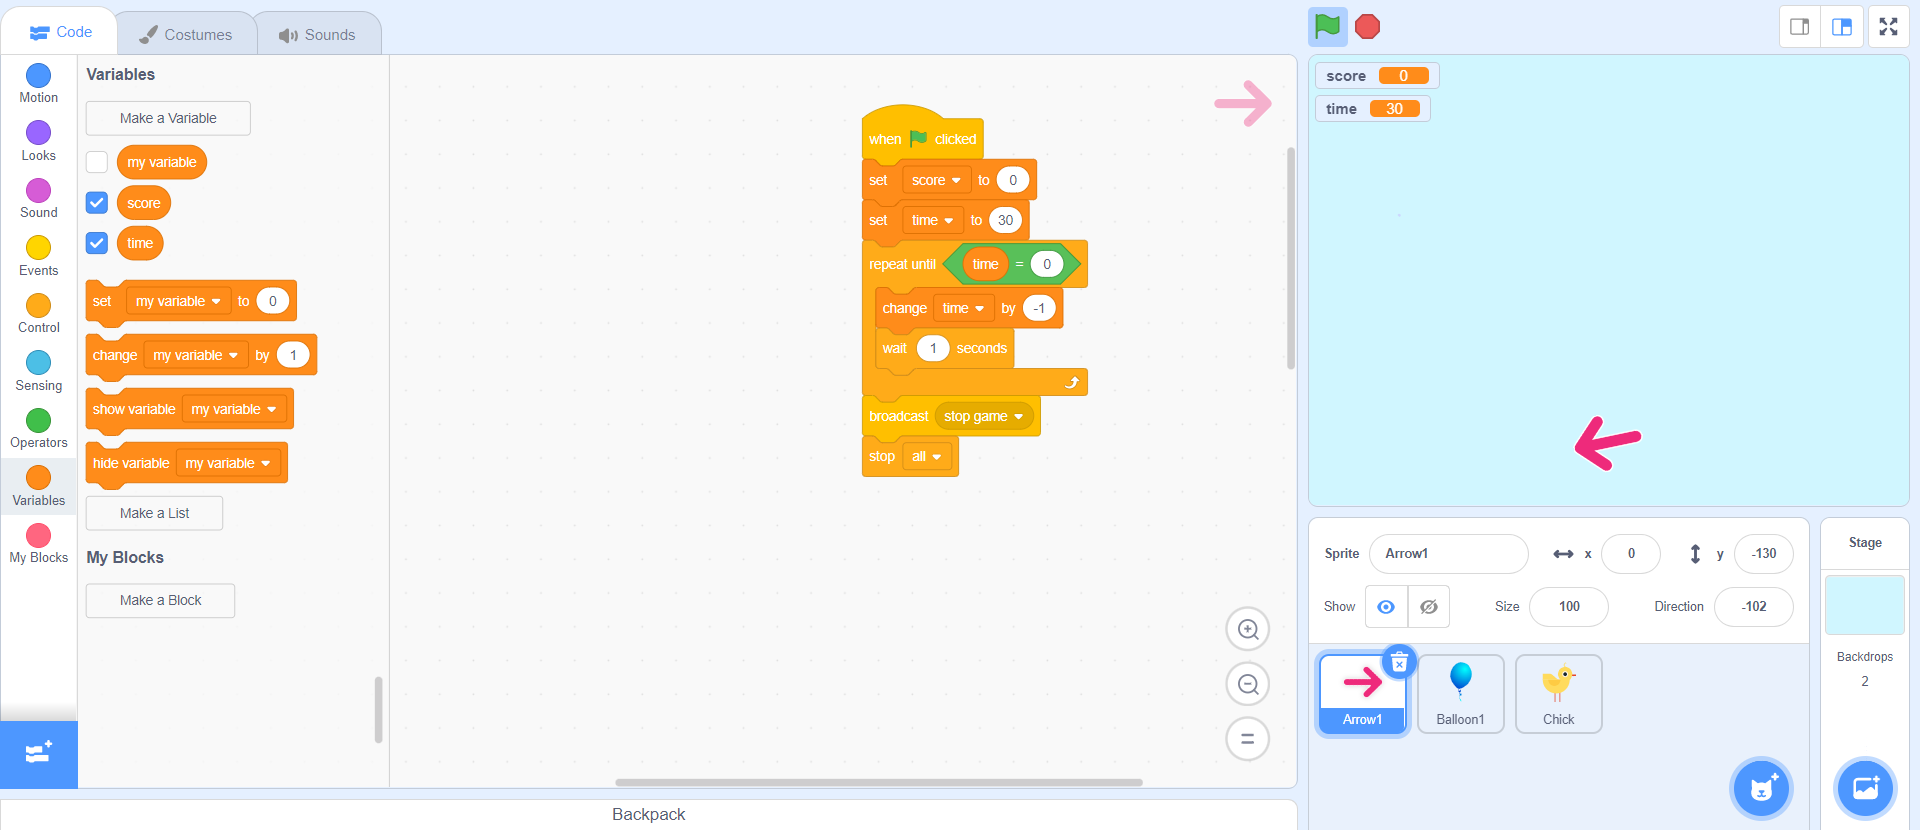
\includegraphics[width=1.0\linewidth,height=0.5\linewidth]{fig090005.png}
  \caption{Изпращане на съобщение за край на играта}
\label{fig090005}
\end{figure}

По време на играта катапулта трябва да бъде позициониран в долната част на екрана и да следва посоката на мишката, докато играчът не кликне с нея. Трябва да се използва вложен цикъл, което означава, че ще има цикъл, който вътре в себе си съдържа друг цикъл. Външният цикъл ще бъде безкраен. Той ще приключи, когато играта приключи. Вътрешният цикъл ще бъде цикъл с цел, като целта е докато не бъде кликнато с мишката. Вътре в тялото на цикъла инструкцията трябва да бъде "point towards mouse-pointer", което означава "следвай мишката".
 
\begin{figure}[H]
  \centering
  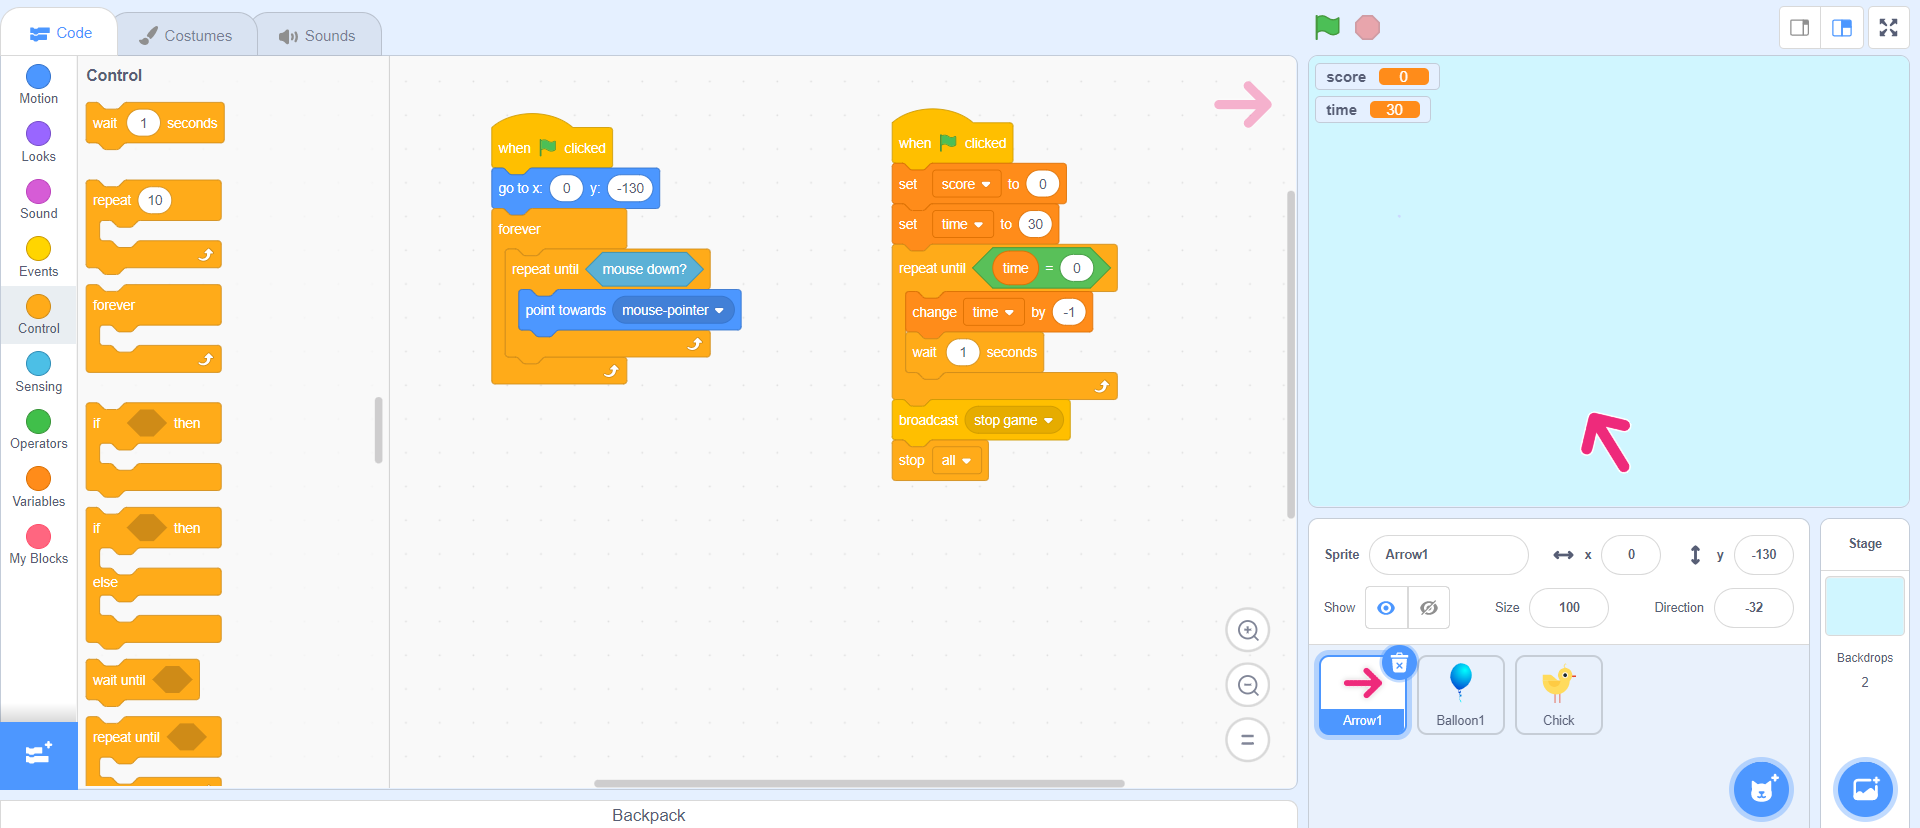
\includegraphics[width=1.0\linewidth,height=0.5\linewidth]{fig090006.png}
  \caption{Проследяване на мишката}
\label{fig090006}
\end{figure}

Когато се стартира играта се забелязва, че катапулта следва посоката на мишката. Това, което остава да се направи е, когато се кликне да се изстреля, а когато докосне някой от ръбовете на екрана да се върне в първоначалното си състояние. Създадено чрез инструкции, това става, като се добави още един вътрешен цикъл. Този път условието на този цикъл трябва да бъде - докато катапулта не докосне някой ръб на екрана. А в тялото на цикъла трябва да се постави инструкцията - движи се с 20 стъпки. Инструкциите извън този цикъл се изпълняват когато героят докосне ръба. За това последната инструкция е да се позиционира героя в начална позиция.

\begin{figure}[H]
  \centering
  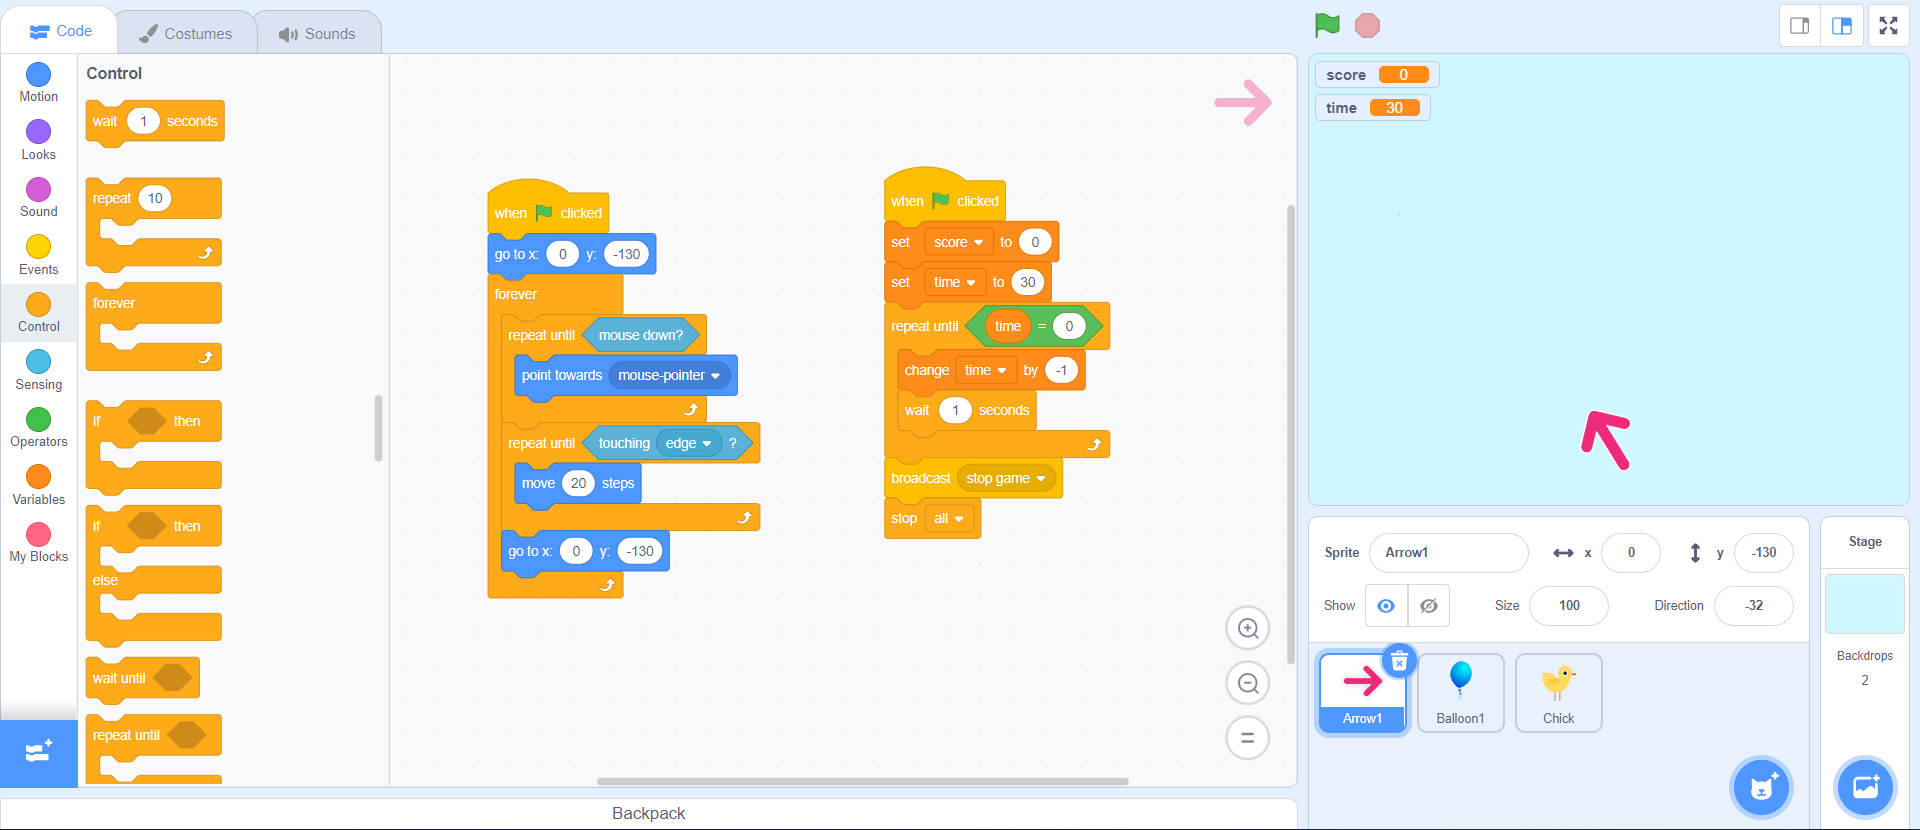
\includegraphics[width=1.0\linewidth,height=0.5\linewidth]{fig090007.png}
  \caption{Финален код на катапулта}
\label{fig090007}
\end{figure}

\section{Програмиране на балона}
В следващата стъпка ще се конструират и инструкциите за балона. По време на играта се появяват много балони, а героят е само един. Това става, като се добавят инструкции за клониране на героя балон. Инструкциите, които ще са необходими за клониране се намират в оранжевата група и са "create clone of myself", което означава "направи клонинг на мен" и инструкцията "delete this clone", което означава "изтрий този клонинг".

Когато играта започне оригиналният герой балон трябва да се скрие. Неговата единствена цел е да създава клонинги. Нека балонът да създава 10 клонинги на себе си, след което да изчаква 5 секунди и да изтрива един клонинг. Този алгоритъм трябва да се повтори 5 пъти. Тук отново трябва да бъде използвана конструкцията - вложен цикъл.

\begin{figure}[H]
  \centering
  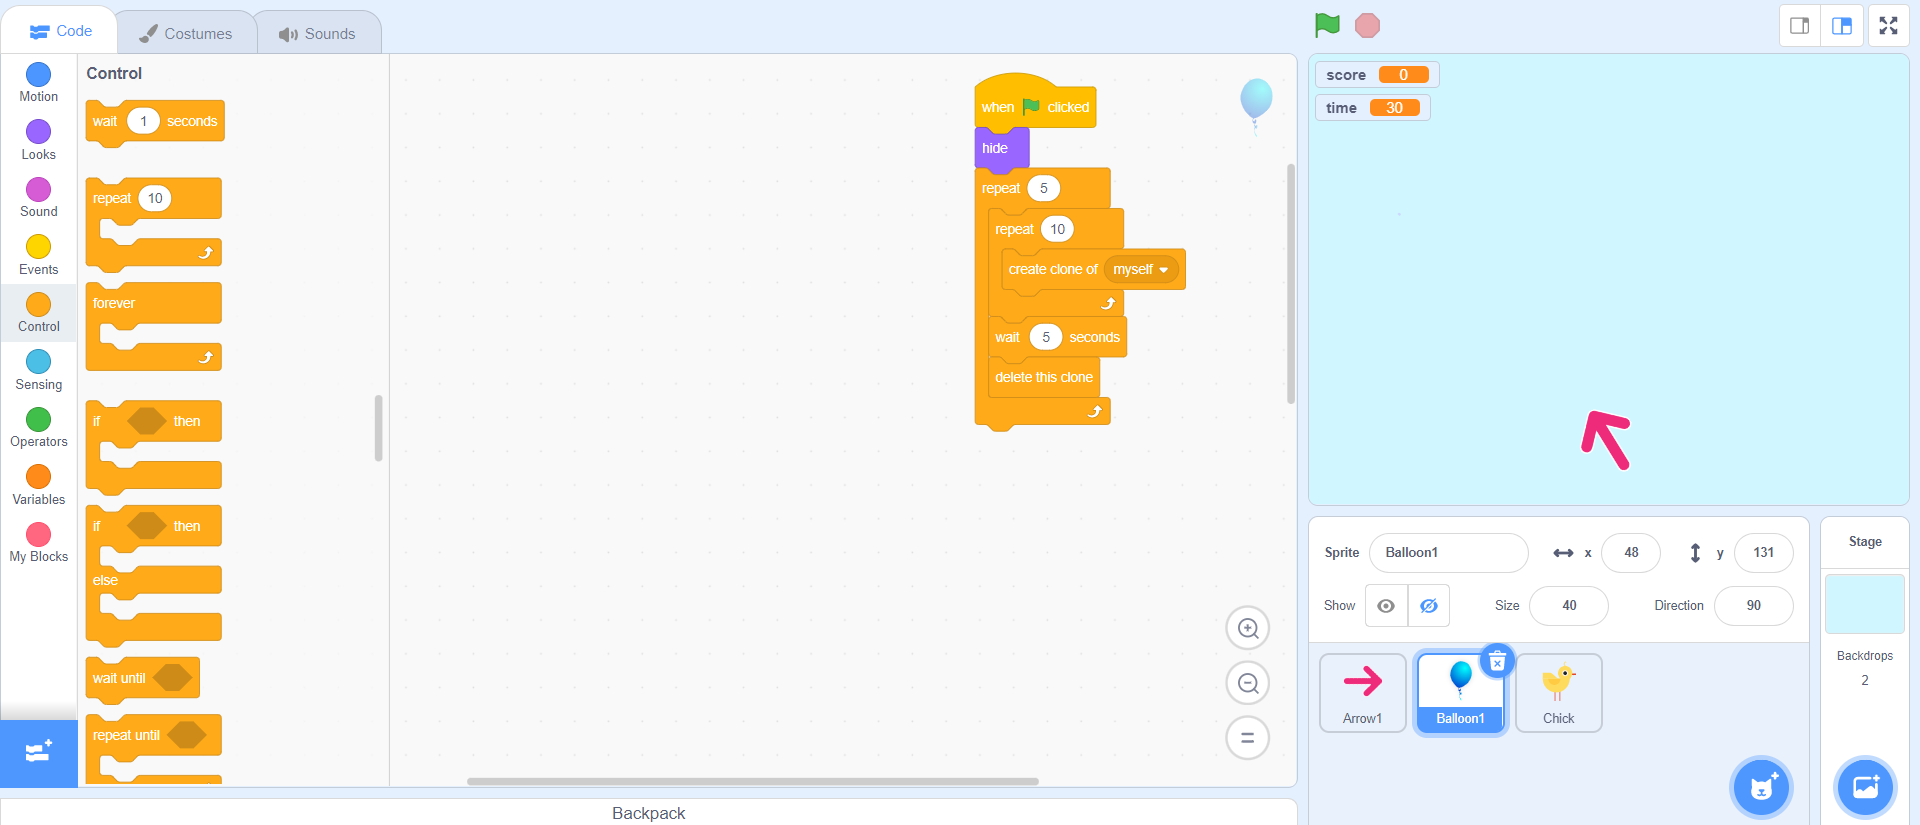
\includegraphics[width=1.0\linewidth,height=0.5\linewidth]{fig090008.png}
  \caption{Създаване на клонинги}
\label{fig090008}
\end{figure}

Следва да се програмира и клонинга на балона. От оранжевата група трябва да се използва инструкцията "When I start as a clone", което означава "Когато стартирам, като клонинг". Първото нещо, което трябва да се направи е да се позиционира клонинга. За да бъде по интересна играта нека позицията му да бъде на случаен принцип, но да бъде в горната част на екрана. Това означава, че числото за координатата x трябва да бъде случайно между -200 и 200 (това са границите на екрана), а за y координатата трябва да бъдат между 50 и 150 (горната част на екрана).

След като се позиционира клонинга следва да се покаже и да се промени размерът му да бъде по- малък. Двете инструкции се намират в лилавата група с инструкции.

\begin{figure}[H]
  \centering
  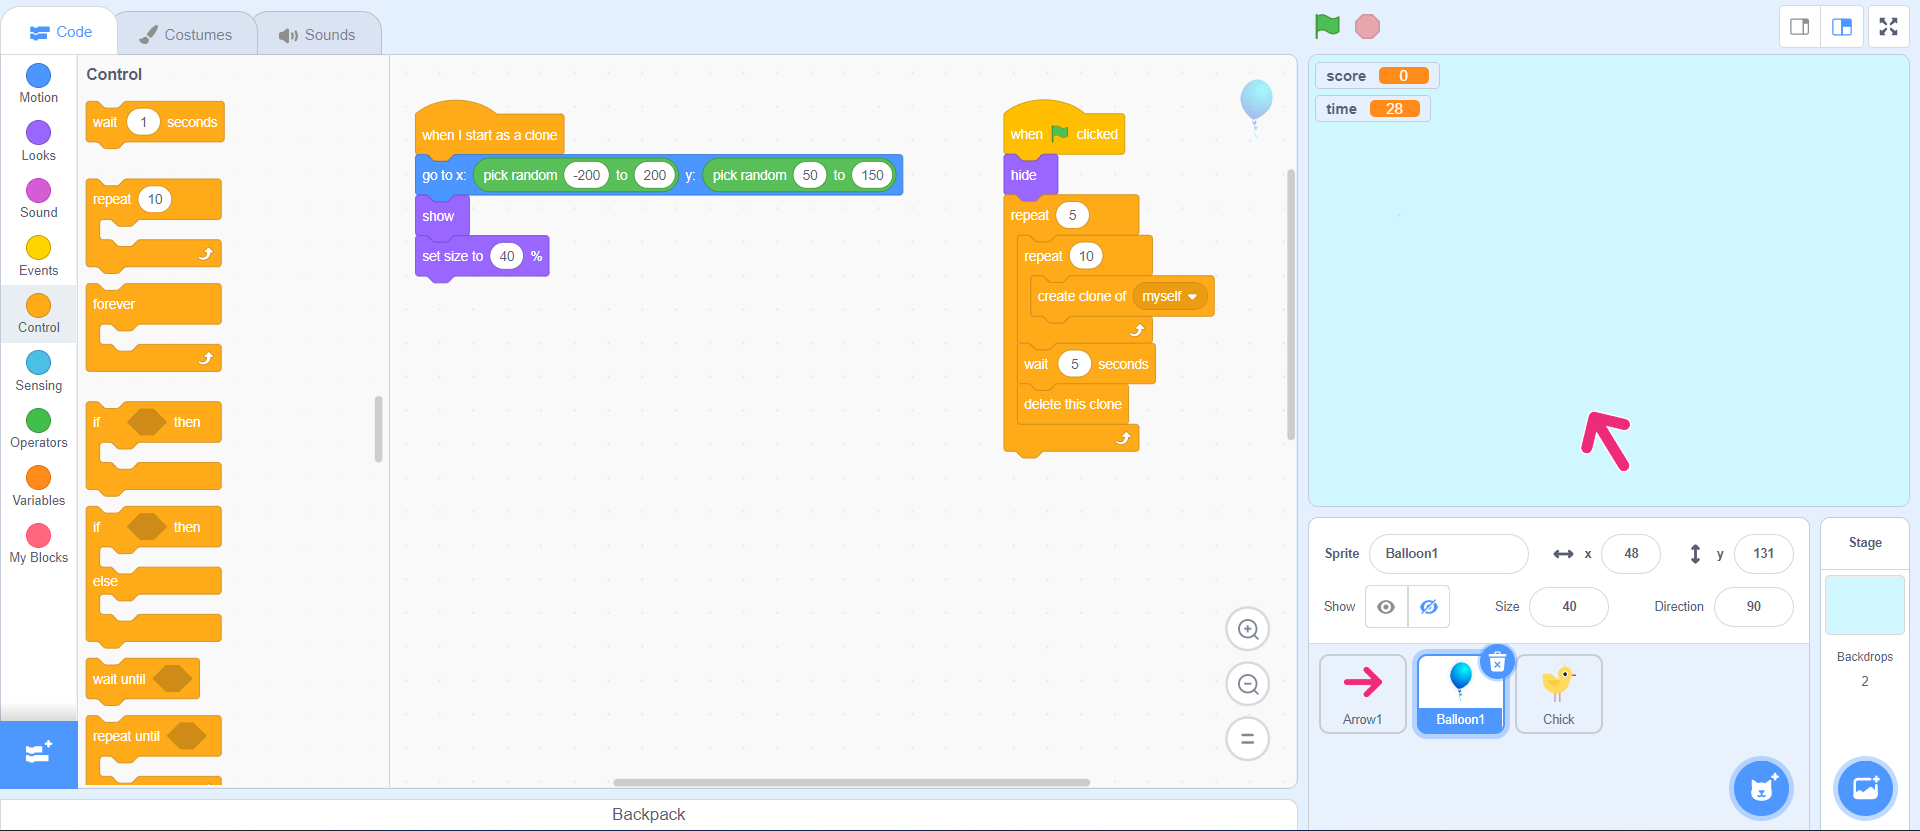
\includegraphics[width=1.0\linewidth,height=0.5\linewidth]{fig090009.png}
  \caption{Позициониране на клонинга}
\label{fig090009}
\end{figure}

След като се появи балонът той трябва да се придвижи с една стъпка. Освен движението на балона трябва да се направят и две проверки. Едната проверка е за това дали стрелката не е докоснала клонинга. Ако условието е вярно, то тогава трябва стойността на променливата за резултата трябва да се увеличи с 1 и отново да се постави балонът на случайна позиция.

\begin{figure}[H]
  \centering
  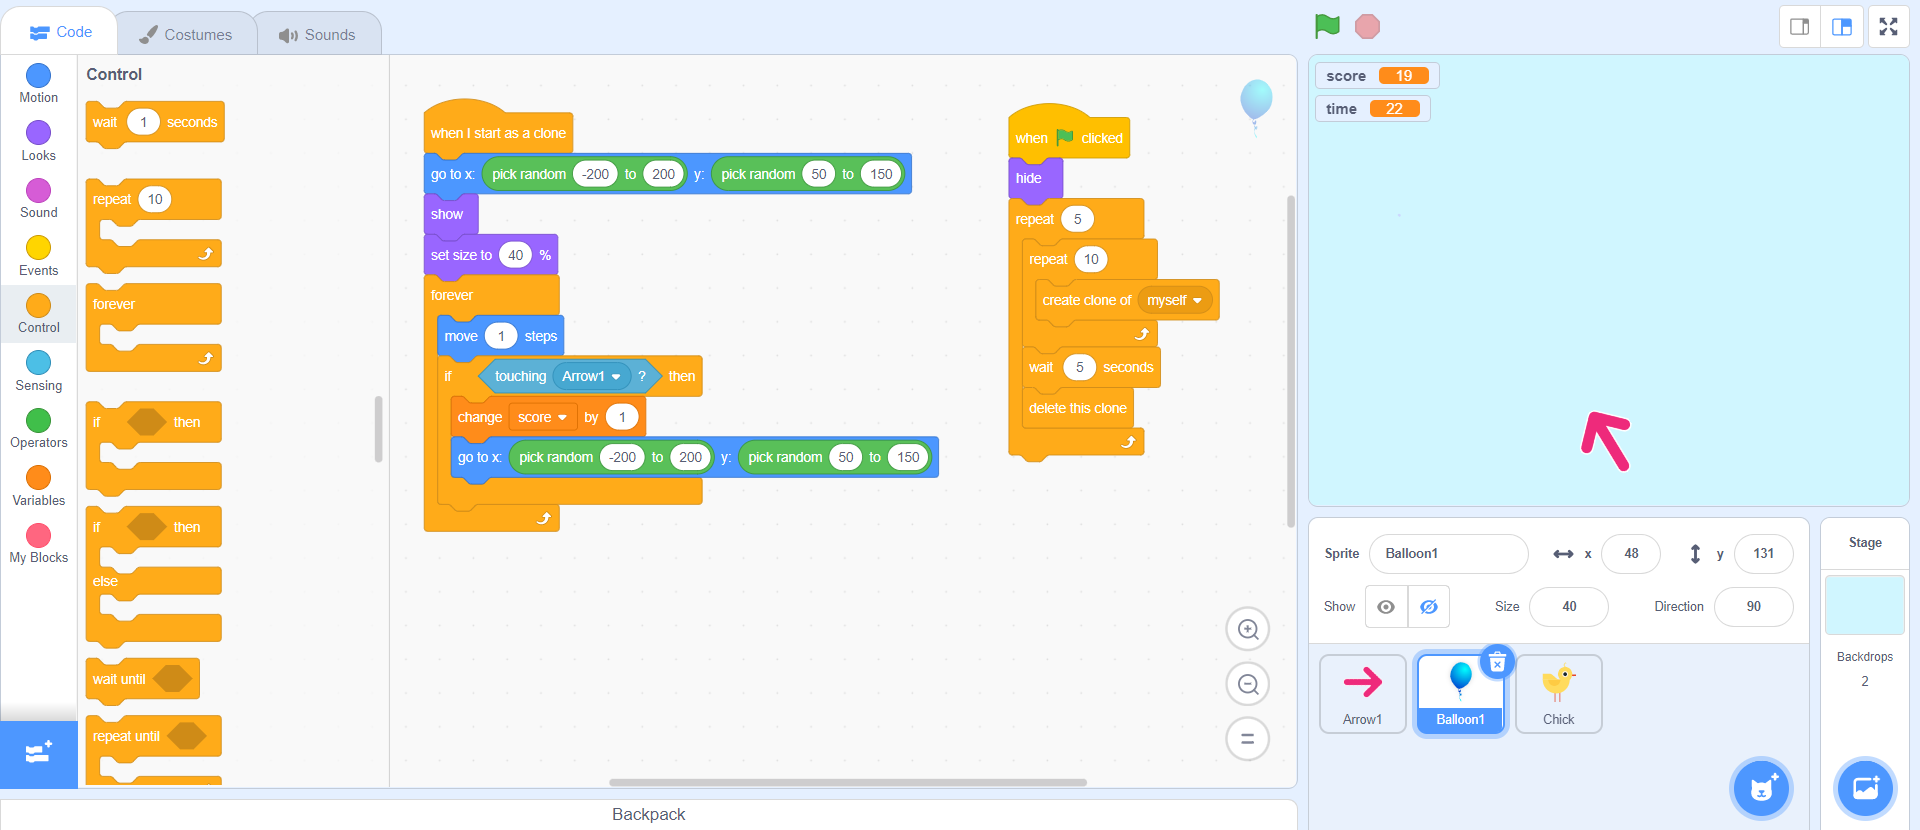
\includegraphics[width=1.0\linewidth,height=0.5\linewidth]{fig090010.png}
  \caption{Увеличаване на резултатът}
\label{fig090010}
\end{figure}

Втората проверка, която трябва да се направи е, ако балонът не е бъде уцелен от катапулта и достигне до края на екрана. Трябва да се провери дали x координатата е по- голяма от 220. Ако условието е вярно, то тогава клонинга трябва да се постави в лявата част на екрана и за да е по- интересна играта ще смени и костюма си (цвета си).

\begin{figure}[H]
  \centering
  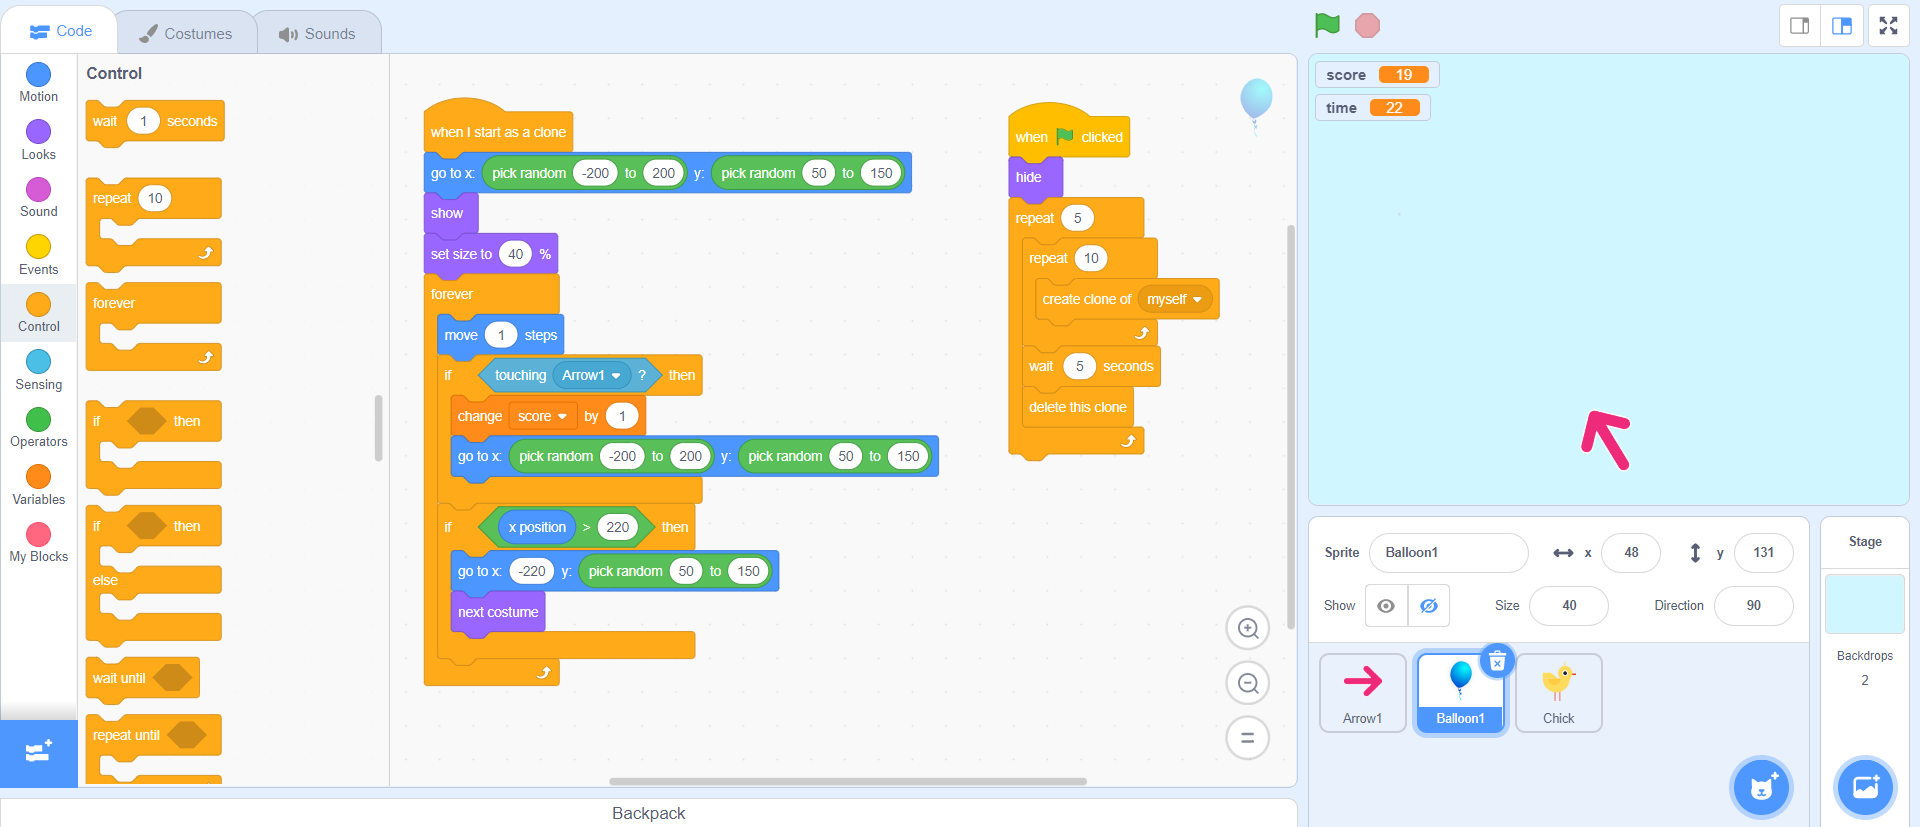
\includegraphics[width=1.0\linewidth,height=0.5\linewidth]{fig090011.png}
  \caption{Кодът на балона}
\label{fig090011}
\end{figure}

Играта е почти готова. Когато се стартира се появяват клонингите на балона и може да бъдат спукани с помощта на катапулта. Също така променливата за време намалява, а тази за резултатът се увеличава.

Последната стъпка, която трябва да се направи е да се програмира героят, който да съобщи крайният резултат. Когато играта започне този герой трябва да бъде скрит. Той трябва да се покаже, когато получи съобщението от катапулта "stop game". Инструкцията, която ще изпише резултатът е от лилавата група - "thing Hmm... for 2 seconds". На мястото на съобщението "Hmm..." трябва да се покаже резултатът. От зелената група с инструкции, инструкцията "join apple banana" залепва двете думи. В тази игра отново трябва да се залепят две неща. Едното е съобщението "Your score is ", а второто е стойността на променливата score.

\begin{figure}[H]
  \centering
  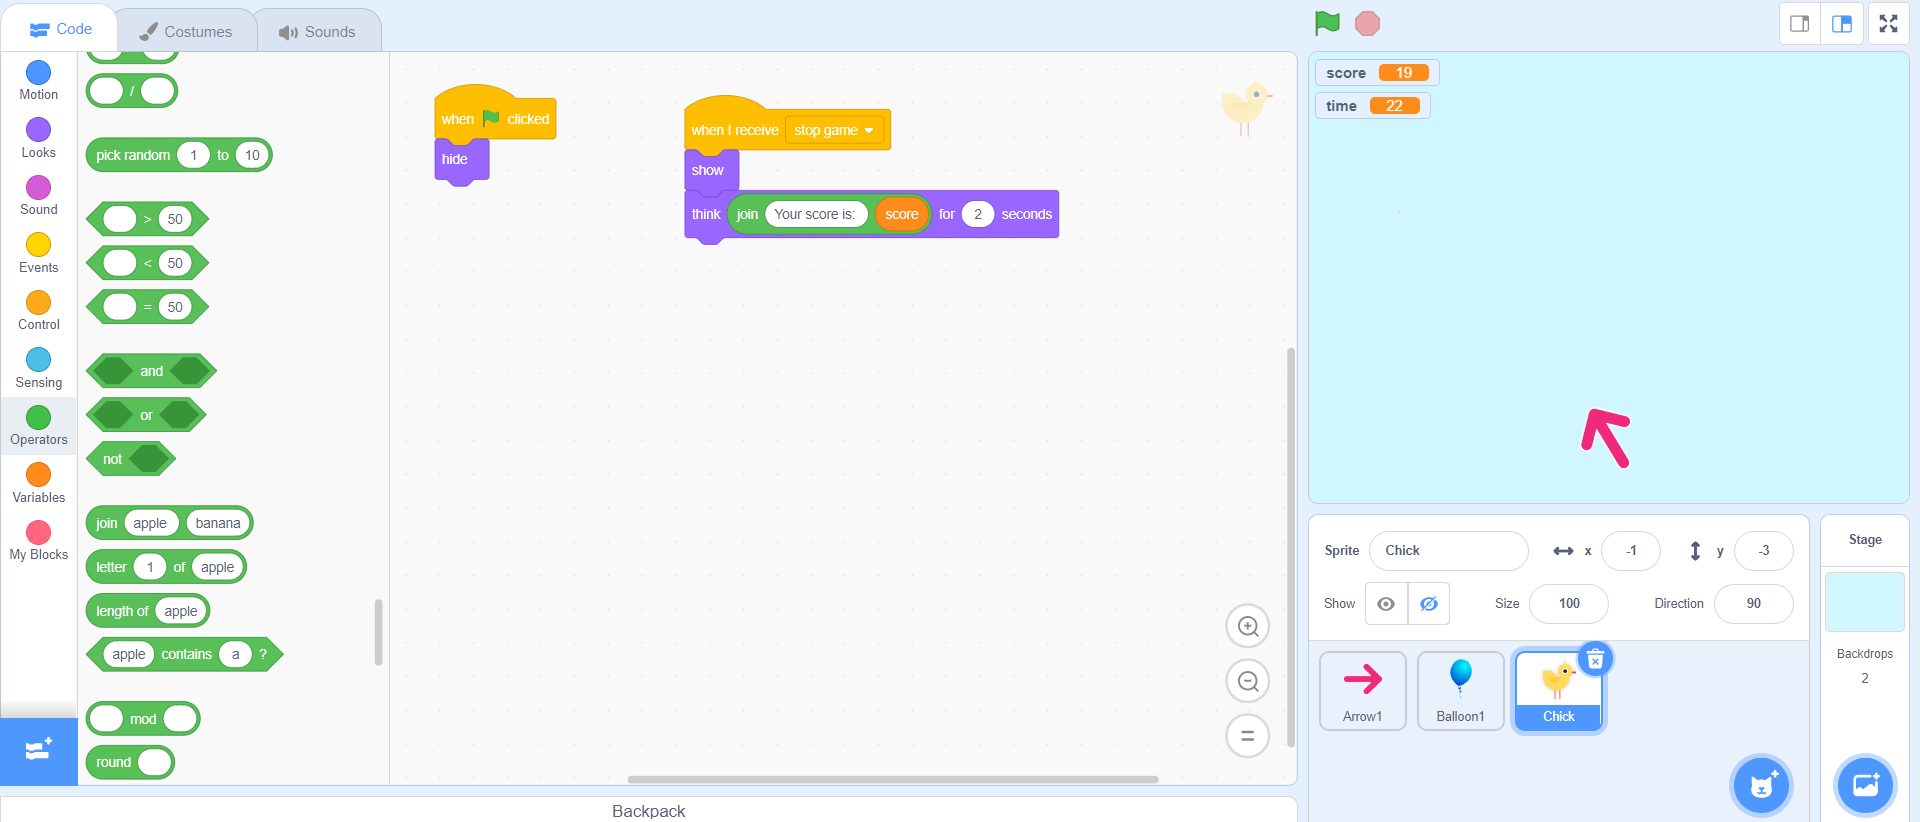
\includegraphics[width=1.0\linewidth,height=0.5\linewidth]{fig090012.png}
  \caption{Кодът на героят, който обявява резултатът}
\label{fig090012}
\end{figure}

Играта е завършена. Играйте я заедно с вашите приятели, за да премерите сили, който от вас ще спука най- много балони за 30 секунди.